\chapter{Metode og Proces}
\valdemar{Mangler quort indledning}
\section{Metode}

Projektgruppen har benyttet scrum som arbejdsmetode, hvori der er lavet 2 ugers sprints. I starten af disse sprints, blev der lavet sprint goals, og planning poker. Ud fra det timeantal som blev vurderet til sprint goals, blev de fordelt så ligelidt som muligt blandt gruppens medlemmer. Når man var tildelt en opgave, arbejdede man oftest også videre med samme kategori i næste sprint. \newline
I slutningen af et sprint, blev der opsamlet på det arbejde man hver især havde opfyldt, og hvis der evt. var opstået problemer undervejs, som skulle løses i næste sprint.
\valdemar{Nævn versionsstyring, SYSML UML}

\valdemar{Scrum, arbejdsprocess, Agil programmering}

\section{Proces} \thomas{noget om product owner}
 Gruppen for dette projekt består af 7 IKT-studerende på 4.semester og 1 vejleder, hvor alle medlemmer kan ses i tabel \ref{tab:grpMedlem}.


\begin{table}[H]
    \centering
    \begin{tabular}{|p{2.2in}|p{1in}|} \hline 
        \textbf{Navne} & \textbf{Studie nr.} \\ \hline 
        Florent Avdjaj & 201409781 \\ \hline 
        Jonathan Fabricius L\"{u}demann & 201404083 \\ \hline 
        Thomas M{\o}ller & 201706260 \\ \hline 
        Mathias Nortvig Thomassen & 201706287 \\ \hline 
        Tobias S{\o}ndergaard M{\o}nster & 201604599 \\ \hline 
        Mathias Nielsen & 201700317 \\ \hline 
        Valdemar Tr{\o}jg{\aa}rd Tang & 201707689 \\ \hline 
        \multicolumn{2}{|l|}{Vejleder:                                                              Lars Mortensen} \\ \hline 
    \end{tabular}
    \caption{Tabel af gruppens medlemmer og gruppens vejleder}
    \label{tab:grpMedlem}
\end{table}

Samarbejdsaftalen blev lavet i begyndelsen af semesterprojektet, hvor gruppemedlemmerne fik en forventningsafstemmelse af hindanden. \valdemar{indsæt refference til samarbejdsaftale.} Der blev snakket om, hvordan projektarbejdet skulle forløbe for gruppemedlemmerne, og hvilke forventninger man har til hinanden for at fuldføre projektet. Gruppen har lagt fokus på at have et godt samarbejde, hvor arbejdet og møder skal tages seriøst, men hvor der samtidig er plads til sjov og fleksibilitet.

Gruppen har arbejdet demokratisk, hvor beslutninger blev diskuteret i gruppen og et valg kom frem, som et resultat af diskussionen. Der har ikke været en decideret leder, dog har rollen som mødeleder/scrum master gået på skift i gruppen, da ingen i gruppen havde et nært ønske om at være leder for gruppen. Da mente gruppen at rollen skulle gå på skift, og alle fik prøvet at arbejde med forskellige roller. Dog gjorde det ikke en stor forskel, hvem der var leder, da beslutningerne blev taget demokratisk. I gruppen blev der også diskuteret om, hvem der skulle være product owner. Det landte på gruppen som helhed, da det var én af gruppens medlemmer der fik idéen til WePlanner.  

I projektet har arbejdsfordelingen til gruppemedlemmer fungeret, da alle kunne vælge hvilke arbejdsopgaver de ville lave. Dog har der været gange, hvor bestemte opgaver var taget af andre. 2w

Til dette projekt er principperne for scrum \cite{Scrum} blevet overholdt efter bedste evne. Der har ikke været mulighed for at mødes hver dag og afholde korte møder, grundet andre kurser på semesteret. Gruppen har holdt sprints af 2 uger, hvor implementeringen i det indeværende sprint,  blev demonstreret for vejleder. Hver gang et nyt sprint startes, er nye sprint-goals blevet diskuteret på gruppen, og opgavernes omfang vurderet ved brug af planning-poker. Hvis en person har haft brug for hjælp til en opgave, er der andre fra teamet der har trådt til.

Til at bevare overblik over projektet og processen, har gruppen benyttet Microsoft Azure DevOps \cite{AzureDevOps} som medium for process arbejde og versionsstyring. Gruppen har brugt Azure Devops\thomas{reference til azure}  til at se backloggen og scrum boardet, hvor work items kunne ses for gruppen. Sprints kunne blive oprettet, hvor et sprint backlog også blev oprettet, så opgaverne for det enkelte sprint kunne ses. Repository for gruppen kunne også findes inde på gruppens side i Azure DevOps, hvor kode og dokumenterne for gruppen findes. Et eksempel på en af gruppens scrum boards for en iteration ses på figur \ref{fig:ScrumBoard}. 
\valdemar{Mangler referencer til process beskrivelsen i bilag}

\begin{figure}[H]
    \centering
    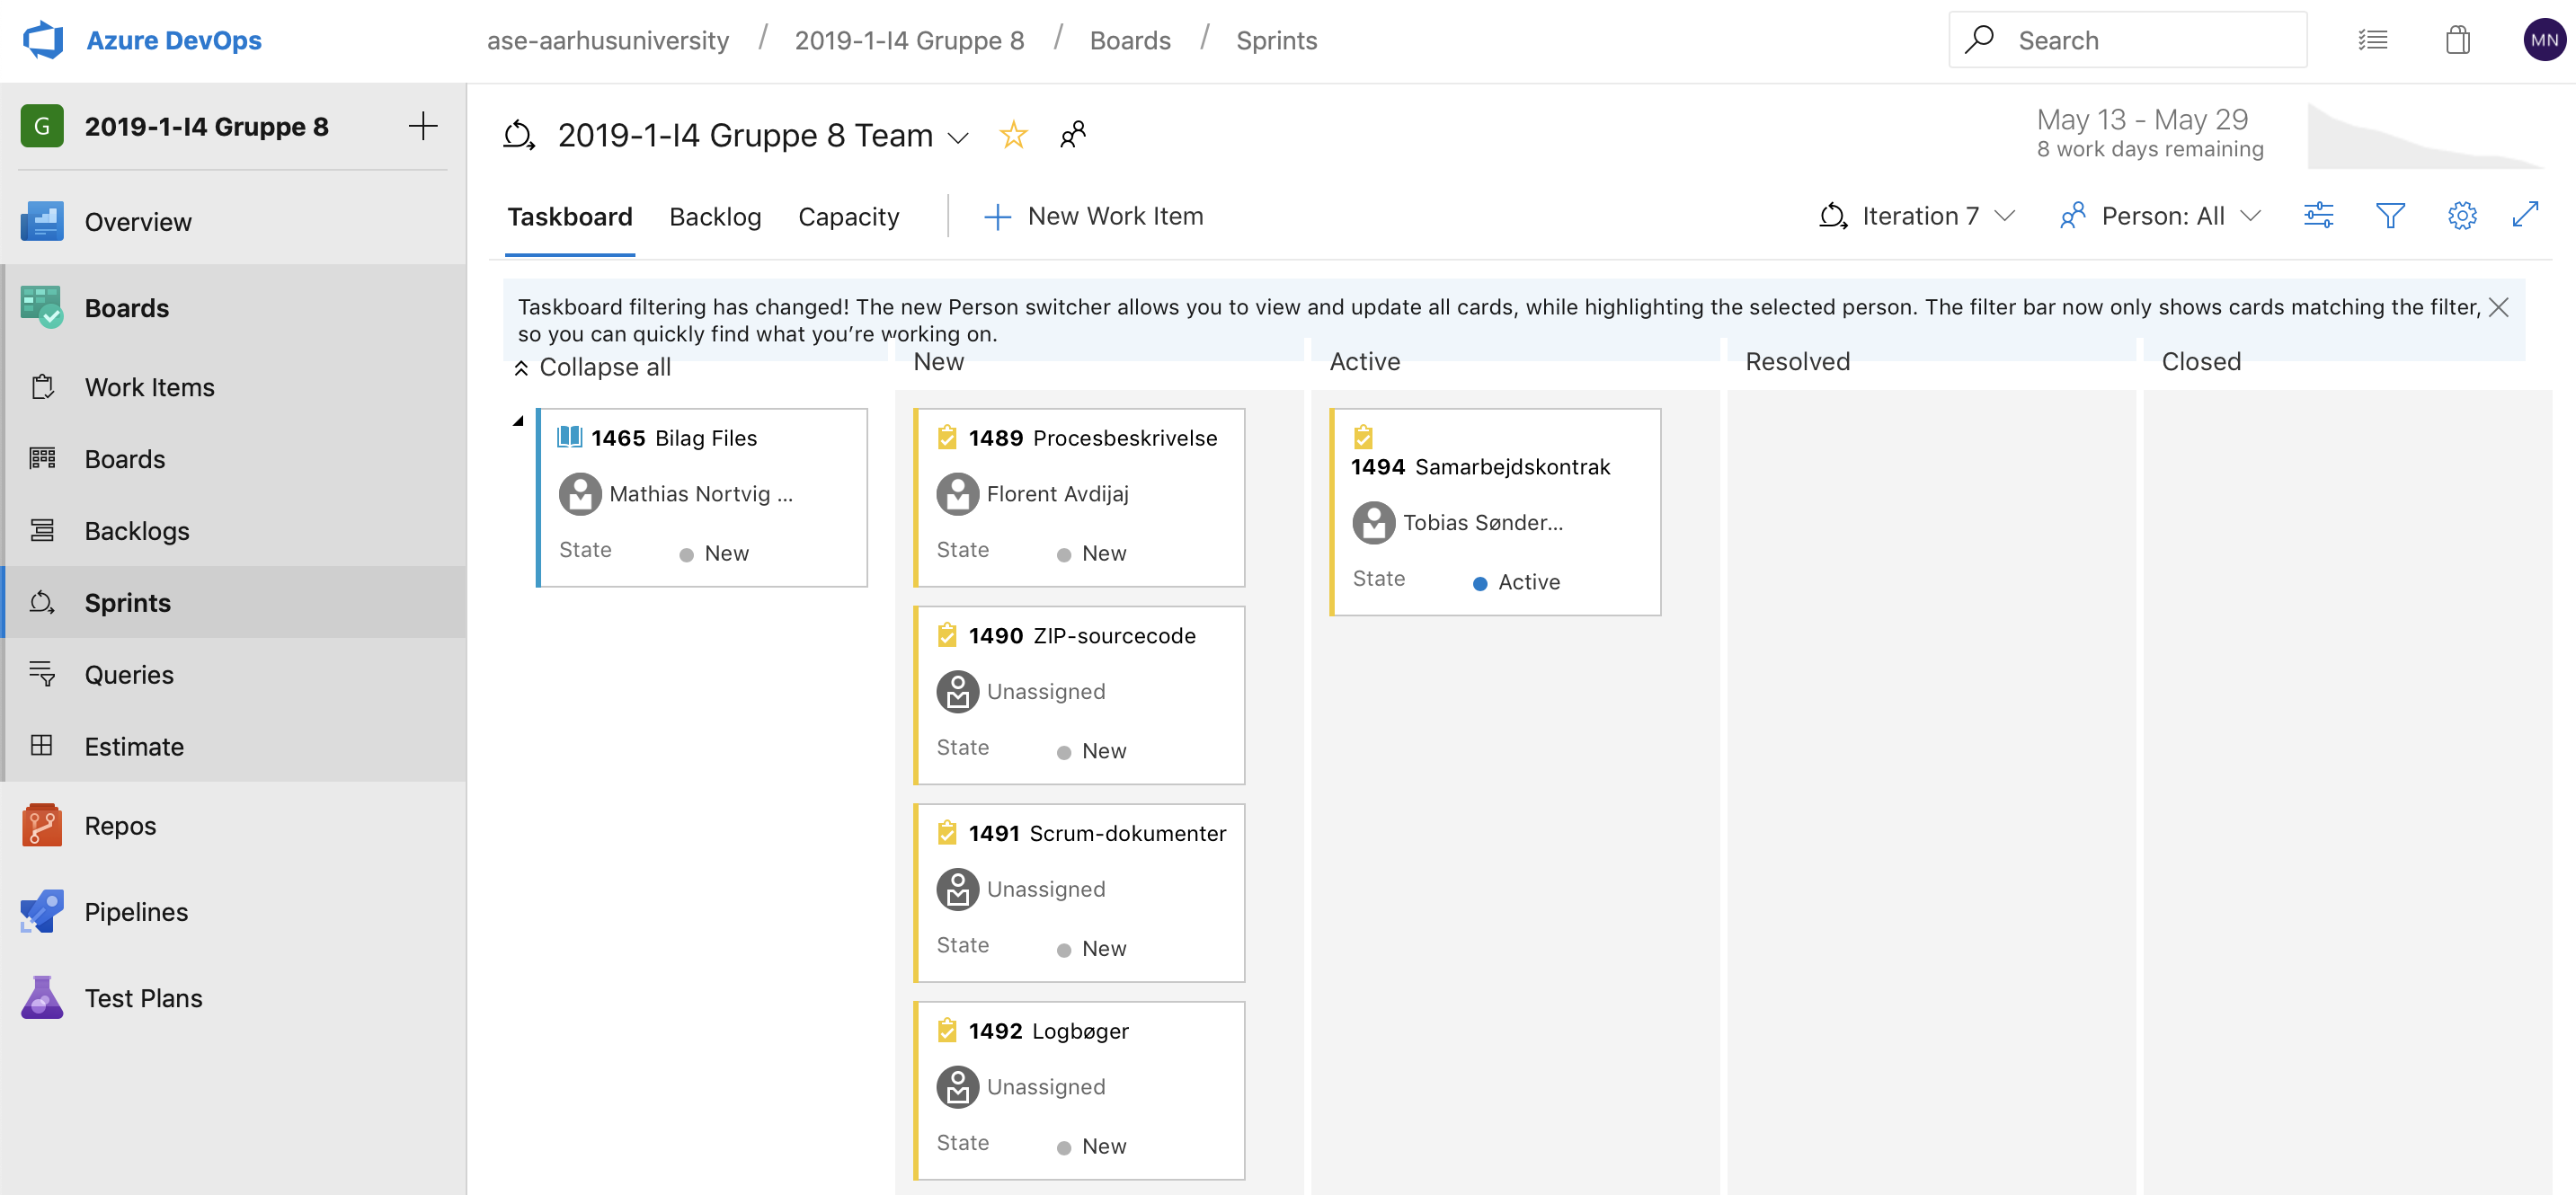
\includegraphics[width=1\linewidth]{07_Metode_og_Proces/Filer/AzureScrumBoard.png}
    \caption{Scrum board for gruppen}
    \label{fig:ScrumBoard}
\end{figure}{}

\subsection{Oversigt over arbejde i iterationerne}
Herunder vises en oversigt over forløbets iterationer, hvor der kort beskrives hvad der er lavet i hver iteration.
\newline \\
\textbf{1. Iteration}
\begin{itemize}
    \item Udarbejdelse af projekt beskrivelse, samt koncept.
    \item Udarbejdelse af US's. 
    \item Afgrænsning og MoSCoW Analyse
    \item Undersøgelse af forskellige teknologier.
\end{itemize}

\textbf{2. Iteration}
\begin{itemize}
    \item Arkitektur, design og implementering af brugerindstillinger samt opslagstavle.
\end{itemize}

\textbf{3. Iteration}
\begin{itemize}
    \item Fortsættelse med arbejde fra 2. iteration, på bruger- og gruppeindstillinger samt opslagstavle.
    \item Satte testprojekt op
    \item Begynde på implementering af liste og gruppeindstillinger
\end{itemize}

\textbf{4. Iteration}
\begin{itemize}
    \item Tilføje validering om brugere har adgang. 
    \item Indledende implementering for Booking og kalender.
    \item Fortsat implementering af List.
\end{itemize}

\textbf{5. Iteration}
\begin{itemize}
    \item Fortsat implementering af Booking, kalender og list.
    \item Start på dashboard siden og widgets.
    \item Start på implementering af planlægning.
\end{itemize}

\textbf{6. Iteration}
\begin{itemize}
    \item Fortsat implementering af dashboard, booking og planlægning
    \item Oprettelse af views til widgets for hver widget-type.
    \item Indledende implementering af betaling.
    \item Implementering af pop-up vinduer for views der opretter/sletter eller redigerer entiteter.
    \item Begyndelse af rapport skrivning
\end{itemize}

\textbf{7. Iteration}
\begin{itemize}
    \item Afsluttende implementering og mindre bug-fixes for alle widgets.
    \item Skrivning af rapport og bilag
\end{itemize}